\section{Loudspeaker}

As previously stated, distortion also occurs in the woofer block in \autoref{fig:speaker_block}. In order to understand how the distortion occurs in a loudspeaker, it is necessary to understand the basic fundamentals and the topology of a loudspeaker. This section will consist of the basic topology and then glans over the topic of vibration induced in the speaker woofer.

%\subsubsection*{The basics}
The loudspeaker is a transducer which purpose is to convert the electrical energy into acoustical energy. This is done by sending the signal into the speaker which can consist of numerous driver. Each driver is made with a specific purpose for handling frequency. The drivers are designed to perform best within their frequency range, hence they are usually different sizes in diameter.
\begin{itemize}
\item[] For the high frequencies their is a tweeter, 1-2 inches in diameters, high frequencies is roughly 3-4 kHz and above.
\item[] In the midrange their is a midrange driver which usually is around 5-6 inches. The midrange is roughly 300 Hz to 3-4 kHz. 
\item[] The lower frequencies, which is 300 and below, is then handled by the woofer. The woofer can is usually 5-6+ inches in diameter.
\end{itemize}
The reason for different diameters in drivers is because of the wavelength the specific frequencies got. Should a woofer play frequencies at +4 kHz it would end in the driver physically not being able to move that fast. The limitations will end up in non-linear distortion in the diaphragm. Vice versa, should a tweeter reproduced low frequency sound at high \gls{SPL} it will end in distortion. The tweeter has a very low excursion range which limits it to the high frequency area.

\todo[inline]{Måske noget forklaring om det kun er nødvendigt at kigge på wooferen}


\subsection{Diaphragm excursion}

When the speaker plays sound it does so by moving the diaphragm in the woofer. This difference in air pressure is then perceived as sound. The sound have a specific wavelength according to the frequency. This means that trying to move the air with a speaker cone is more efficient in a specific frequency area according to the diameter. %If a speaker with a small diameter tries to generate a large wavelength the sound would bend and escape around the edges. 
Since a large wavelength requires more air to be pushed. Hence we need different sizes of speaker cones which is sized according to what area they are going to play.

Next, the woofer needs to deliver a sufficient \gls{SPL}. This creates the need for a enough excursion of the diaphragm. Without dwelling to much on the speaker construction, the diaphragm is suspended in free air hold in place by the surround, see \autoref{fig:regularspeaker}, and the spyder. The spyder is a diaphragm holding the voice coil more tightly in place. When the diaphragm moves it will have physical limits from the mechanical construction. At most, the diaphragm will move regular and linear. When the diaphragm is pushed to the boundaries, the limits of the mechanical construction will intervene and create non-linearities and distortion. This is discussed further in \autoref{subsec:impulses}.

\begin{figure}
\centering
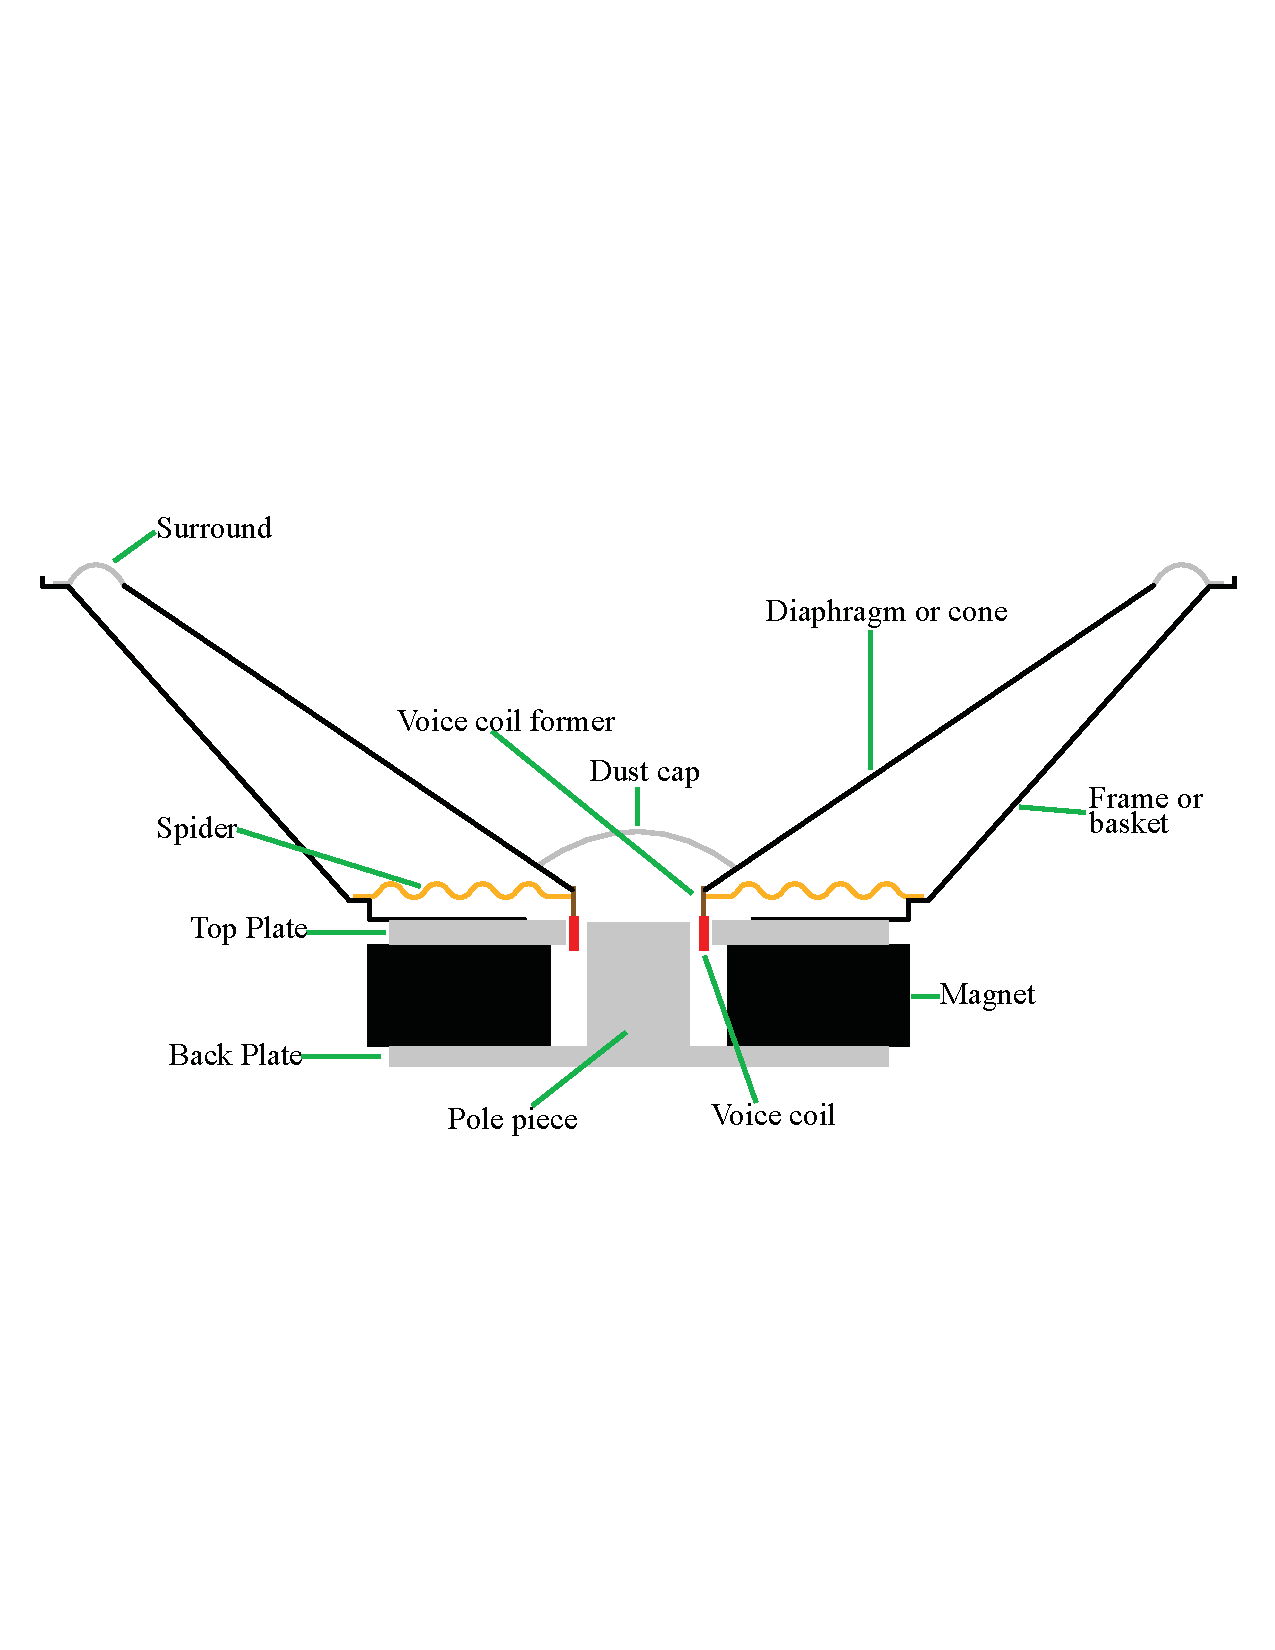
\includegraphics[width=0.75\textwidth]{Speaker-cross-section}
\caption{Cross section of a woofer}
\label{fig:louderspeakerCrossSection}
\end{figure}



\subsection{Impulses}\label{subsec:impulses}
%
%A common problem when designing loudspeakers are the vibrations from the enclosure. If the vibrations are strong, they will become audible and distort the overall sound. The sound radiation from the enclosure will become greater when the \gls{SPL} from the speaker increase. This problem is solved with different techniques but yield more or less the same outcome, which is stiffening of the enclosure. Some of the techniques for removing vibrations from the enclosure could be:
%\begin{itemize}
%\item Mechanical decoupling of the drivers from the enclosure.
%\item Denser or heavier construction material with a high natural frequency, making it harder for the enclosure to start vibrating.
%\item Dampening material or complex structural design inside the cabinet to disperse the sound.
%\end{itemize}
%\todo[inline]{Skal nok lige skaffe nogle kilder på de udtagelser}
%
%Another possibility is to use the vibration measurement as an indicator to tell the current performance of the loudspeaker. Since the loudspeaker will vibrate more at higher volumes. 
%
%
%Looking further into the woofer itself, it shows in \autoref{fig:SpeakerModelStress} that parts in the woofer also creates unwanted vibrations. The purpose of the woofer is to reproduce the electrical signal as an acoustical signal. This is done by using a diaphragm which is suspended in a very light and easy to move material. An Induction in the coil is created in a permanent magnet creating a a electro magnetic force resulting in the diaphragm moving. The goal will always be to loose as little as possible energy, giving the most perfect output. The woofer simply needs to be as powerful, light, stiff and efficient as possible.
%
%\begin{figure}[H]
%\centering
%\begin{subfigure}[t]{0.47\textwidth}
%\includegraphics[width=\linewidth]{SpeakerGOOD}
%	\caption{Regular speaker driver showing surround, diaphragm and the magnet.}
%	\label{fig:regularspeaker}
%\end{subfigure}
%\hspace{6mm} 
%\begin{subfigure}[t]{0.47\textwidth}
%\includegraphics[width=\linewidth]{SpeakerBAD}
%	\caption{Regular speaker driver with red markings showing stress areas}
%	\label{fig:badspeaker}
%\end{subfigure}
%\caption{A Speaker driver, where \ref{fig:badspeaker} shows the stress points outlined with red.}
%\label{fig:SpeakerModelStress}
%\end{figure}
%%When this signal has a large amplitude, read overload, the diaphragm reaches physical capacity. 
%In \autoref{fig:badspeaker} it shows that when a diaphragm is pushed to its maximum capacity the surround will affect the diaphragm causing unwanted distortion. This will be one of the major problems if the diaphragm is not sufficiently stiff to withstand the high \gls{SPL} and not twist during playback. 

Another notice is the coil hitting the back plate. This would again result in distortion since the coil is now hitting the absolute furthest position possible. This situation can however be resolved by moving the back plate further back. This would make the surround determine how far the diaphragm can be pushed.

% \begin{figure}[H]
% \centering
% \tikzsetnextfilename{Impulse1}
% \scalebox{0.7}{
% % This file was created by matlab2tikz.
%
%The latest updates can be retrieved from
%  http://www.mathworks.com/matlabcentral/fileexchange/22022-matlab2tikz-matlab2tikz
%where you can also make suggestions and rate matlab2tikz.
%
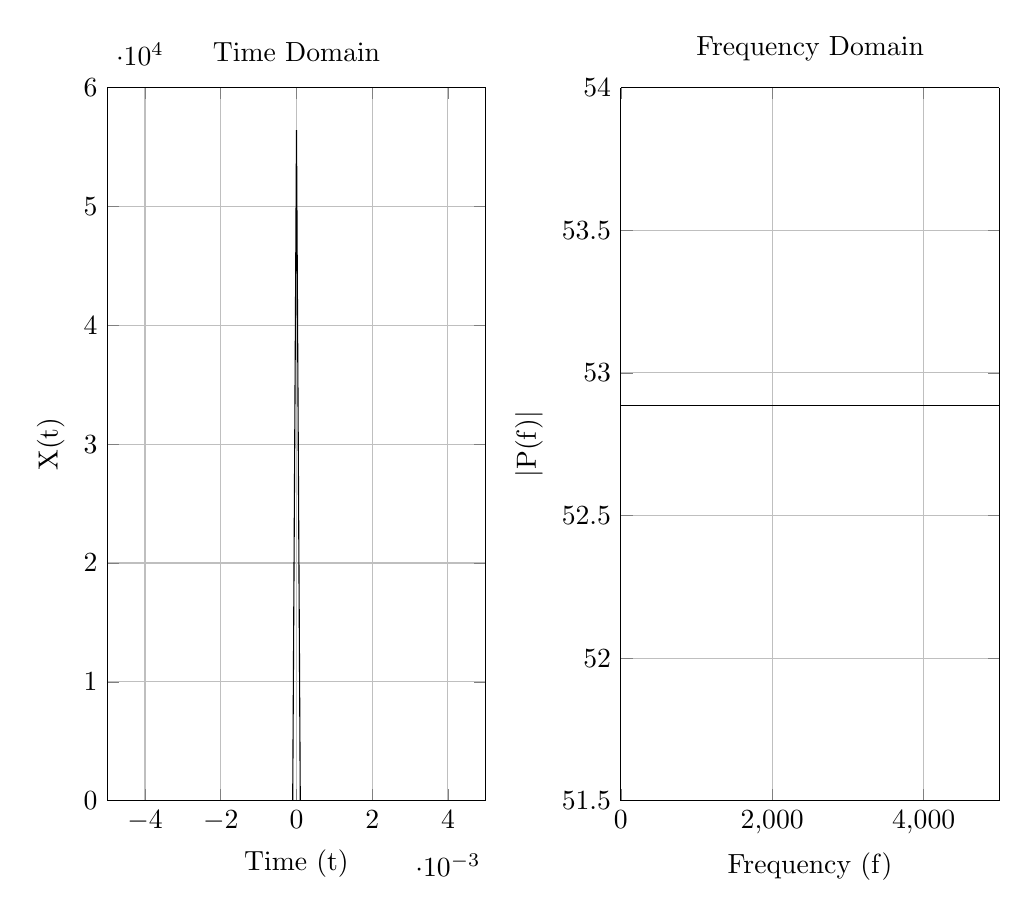
\begin{tikzpicture}

\begin{axis}[%
width=1.893in,
height=3.566in,
at={(0.818in,0.481in)},
scale only axis,
separate axis lines,
every outer x axis line/.append style={black},
every x tick label/.append style={font=\color{black}},
xmin=-0.005,
xmax=0.005,
xlabel={Time (t)},
xmajorgrids,
every outer y axis line/.append style={black},
every y tick label/.append style={font=\color{black}},
ymin=0,
ymax=60000,
ylabel={X(t)},
ymajorgrids,
axis background/.style={fill=white},
title={Time Domain}
]
\addplot [color=black,solid,forget plot]
  table[row sep=crcr]{%
-0.005	0\\
-0.0049	0\\
-0.0048	0\\
-0.0047	0\\
-0.0046	0\\
-0.0045	0\\
-0.0044	0\\
-0.0043	0\\
-0.0042	0\\
-0.0041	0\\
-0.004	0\\
-0.0039	0\\
-0.0038	0\\
-0.0037	0\\
-0.0036	0\\
-0.0035	0\\
-0.0034	0\\
-0.0033	0\\
-0.0032	0\\
-0.0031	0\\
-0.003	0\\
-0.0029	0\\
-0.0028	0\\
-0.0027	0\\
-0.0026	0\\
-0.0025	0\\
-0.0024	0\\
-0.0023	0\\
-0.0022	0\\
-0.0021	0\\
-0.002	0\\
-0.0019	0\\
-0.0018	0\\
-0.0017	0\\
-0.0016	0\\
-0.0015	0\\
-0.0014	0\\
-0.0013	0\\
-0.0012	0\\
-0.0011	0\\
-0.001	0\\
-0.0009	0\\
-0.0008	0\\
-0.0007	0\\
-0.0006	0\\
-0.0005	0\\
-0.0004	0\\
-0.0003	0\\
-0.0002	1.08051873719493e-169\\
-0.0001	2.09882811567613e-39\\
0	56418.9583547756\\
0.0001	2.09882811567613e-39\\
0.0002	1.08051873719493e-169\\
0.0003	0\\
0.0004	0\\
0.0005	0\\
0.0006	0\\
0.0007	0\\
0.0008	0\\
0.0009	0\\
0.001	0\\
0.0011	0\\
0.0012	0\\
0.0013	0\\
0.0014	0\\
0.0015	0\\
0.0016	0\\
0.0017	0\\
0.0018	0\\
0.0019	0\\
0.002	0\\
0.0021	0\\
0.0022	0\\
0.0023	0\\
0.0024	0\\
0.0025	0\\
0.0026	0\\
0.0027	0\\
0.0028	0\\
0.0029	0\\
0.003	0\\
0.0031	0\\
0.0032	0\\
0.0033	0\\
0.0034	0\\
0.0035	0\\
0.0036	0\\
0.0037	0\\
0.0038	0\\
0.0039	0\\
0.004	0\\
0.0041	0\\
0.0042	0\\
0.0043	0\\
0.0044	0\\
0.0045	0\\
0.0046	0\\
0.0047	0\\
0.0048	0\\
0.0049	0\\
0.005	0\\
};
\end{axis}

\begin{axis}[%
width=1.893in,
height=3.566in,
at={(3.386in,0.481in)},
scale only axis,
separate axis lines,
every outer x axis line/.append style={black},
every x tick label/.append style={font=\color{black}},
xmin=0,
xmax=5000,
xlabel={Frequency (f)},
xmajorgrids,
every outer y axis line/.append style={black},
every y tick label/.append style={font=\color{black}},
ymin=51.5,
ymax=54,
ylabel={$|$P(f)$|$},
ymajorgrids,
axis background/.style={fill=white},
title={Frequency Domain}
]
\addplot [color=black,solid,forget plot]
  table[row sep=crcr]{%
0	52.8843018801013\\
78.125	52.8843018801013\\
156.25	52.8843018801013\\
234.375	52.8843018801013\\
312.5	52.8843018801013\\
390.625	52.8843018801013\\
468.75	52.8843018801013\\
546.875	52.8843018801013\\
625	52.8843018801013\\
703.125	52.8843018801013\\
781.25	52.8843018801013\\
859.375	52.8843018801013\\
937.5	52.8843018801013\\
1015.625	52.8843018801013\\
1093.75	52.8843018801013\\
1171.875	52.8843018801013\\
1250	52.8843018801013\\
1328.125	52.8843018801013\\
1406.25	52.8843018801013\\
1484.375	52.8843018801013\\
1562.5	52.8843018801013\\
1640.625	52.8843018801013\\
1718.75	52.8843018801013\\
1796.875	52.8843018801013\\
1875	52.8843018801013\\
1953.125	52.8843018801013\\
2031.25	52.8843018801013\\
2109.375	52.8843018801013\\
2187.5	52.8843018801013\\
2265.625	52.8843018801013\\
2343.75	52.8843018801013\\
2421.875	52.8843018801013\\
2500	52.8843018801013\\
2578.125	52.8843018801013\\
2656.25	52.8843018801013\\
2734.375	52.8843018801013\\
2812.5	52.8843018801013\\
2890.625	52.8843018801013\\
2968.75	52.8843018801013\\
3046.875	52.8843018801013\\
3125	52.8843018801013\\
3203.125	52.8843018801013\\
3281.25	52.8843018801013\\
3359.375	52.8843018801013\\
3437.5	52.8843018801013\\
3515.625	52.8843018801013\\
3593.75	52.8843018801013\\
3671.875	52.8843018801013\\
3750	52.8843018801013\\
3828.125	52.8843018801013\\
3906.25	52.8843018801013\\
3984.375	52.8843018801013\\
4062.5	52.8843018801013\\
4140.625	52.8843018801013\\
4218.75	52.8843018801013\\
4296.875	52.8843018801013\\
4375	52.8843018801013\\
4453.125	52.8843018801013\\
4531.25	52.8843018801013\\
4609.375	52.8843018801013\\
4687.5	52.8843018801013\\
4765.625	52.8843018801013\\
4843.75	52.8843018801013\\
4921.875	52.8843018801013\\
5000	52.8843018801013\\
};
\end{axis}
\end{tikzpicture}%
% }
% \caption{An impulse }
% \label{fig:impulse1}
% \end{figure}

% \begin{figure}[H]
% \centering
% \tikzsetnextfilename{Impulse2}
% \scalebox{0.7}{
% % This file was created by matlab2tikz.
%
%The latest updates can be retrieved from
%  http://www.mathworks.com/matlabcentral/fileexchange/22022-matlab2tikz-matlab2tikz
%where you can also make suggestions and rate matlab2tikz.
%
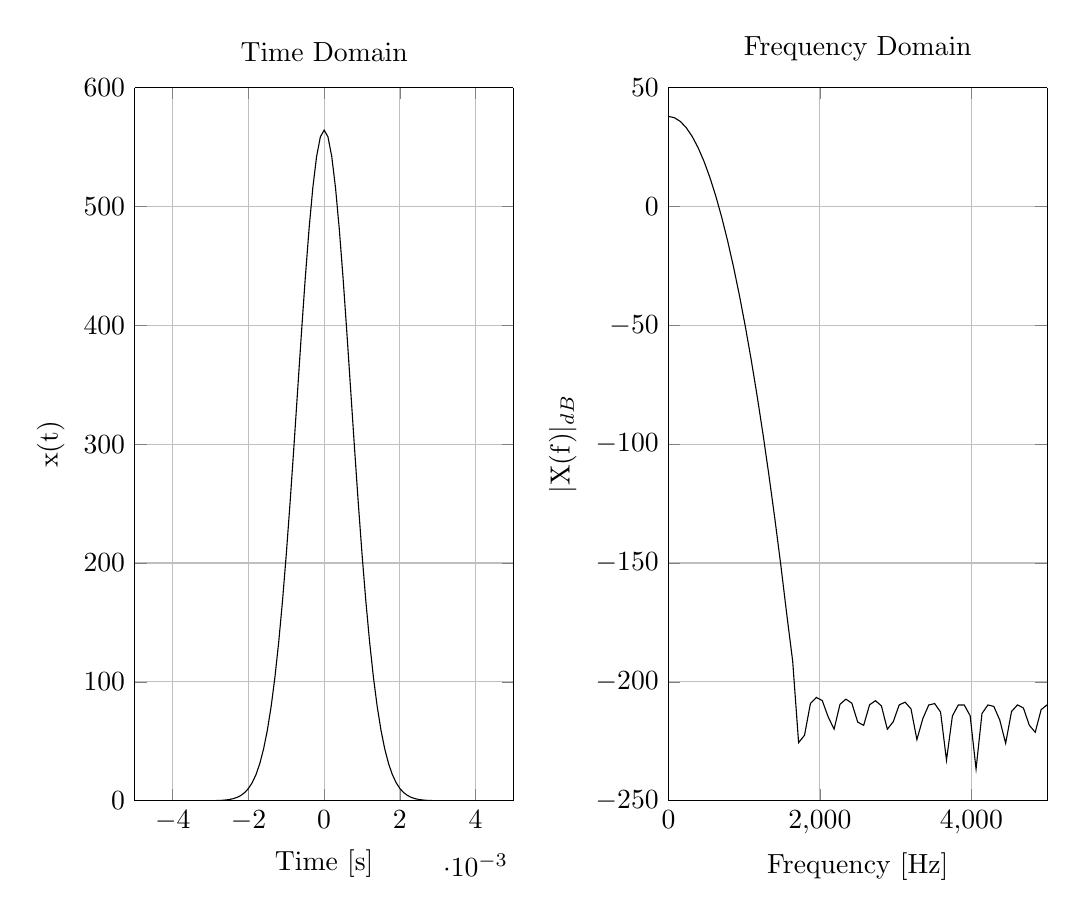
\begin{tikzpicture}

\begin{axis}[%
width=1.893in,
height=3.566in,
at={(0.818in,0.481in)},
scale only axis,
separate axis lines,
every outer x axis line/.append style={black},
every x tick label/.append style={font=\color{black}},
xmin=-0.005,
xmax=0.005,
xlabel={Time [s]},
xmajorgrids,
every outer y axis line/.append style={black},
every y tick label/.append style={font=\color{black}},
ymin=0,
ymax=600,
ylabel={x(t)},
ymajorgrids,
axis background/.style={fill=white},
title={Time Domain}
]
\addplot [color=black,solid,forget plot]
  table[row sep=crcr]{%
-0.005	7.83543326550864e-09\\
-0.0049	2.1086988109929e-08\\
-0.0048	5.56263034490542e-08\\
-0.0047	1.43833470140254e-07\\
-0.0046	3.64547250119098e-07\\
-0.0045	9.05652947954342e-07\\
-0.0044	2.2053823473417e-06\\
-0.0043	5.26405106104077e-06\\
-0.0042	1.23160204933418e-05\\
-0.0041	2.82445606028581e-05\\
-0.004	6.34911733593328e-05\\
-0.0039	0.00013989622447875\\
-0.0038	0.000302143144661123\\
-0.0037	0.000639637042267003\\
-0.0036	0.00132729842235829\\
-0.0035	0.00269971338869239\\
-0.0034	0.00538246051834033\\
-0.0033	0.0105186052217902\\
-0.0032	0.0201488177666178\\
-0.0031	0.0378316333982708\\
-0.003	0.0696265259733739\\
-0.0029	0.125605446260365\\
-0.0028	0.222103972102833\\
-0.0027	0.384962379927571\\
-0.0026	0.654025024861641\\
-0.0025	1.08914211517635\\
-0.0024	1.77782434043888\\
-0.0023	2.84450862126268\\
-0.0022	4.4610775324581\\
-0.0021	6.85782499990342\\
-0.002	10.333492677046\\
-0.0019	15.2623702177239\\
-0.0018	22.0958616660055\\
-0.0017	31.3555202484342\\
-0.0016	43.6145293169727\\
-0.0015	59.4651446118147\\
-0.0014	79.470853838639\\
-0.0013	104.103993398035\\
-0.0012	133.67217350177\\
-0.0011	168.239798896622\\
-0.001	207.553748710297\\
-0.0009	250.984287120181\\
-0.0008	297.492893128735\\
-0.0007	345.637430205269\\
-0.0006	393.621715857144\\
-0.0005	439.391289467723\\
-0.0004	480.770649419654\\
-0.0003	515.630454809482\\
-0.0002	542.067393552432\\
-0.0001	558.575803394468\\
0	564.189583547756\\
0.0001	558.575803394468\\
0.0002	542.067393552432\\
0.0003	515.630454809482\\
0.0004	480.770649419654\\
0.0005	439.391289467723\\
0.0006	393.621715857144\\
0.0007	345.637430205269\\
0.0008	297.492893128735\\
0.0009	250.984287120181\\
0.001	207.553748710297\\
0.0011	168.239798896622\\
0.0012	133.67217350177\\
0.0013	104.103993398035\\
0.0014	79.470853838639\\
0.0015	59.4651446118147\\
0.0016	43.6145293169727\\
0.0017	31.3555202484342\\
0.0018	22.0958616660055\\
0.0019	15.2623702177239\\
0.002	10.333492677046\\
0.0021	6.85782499990342\\
0.0022	4.4610775324581\\
0.0023	2.84450862126268\\
0.0024	1.77782434043888\\
0.0025	1.08914211517635\\
0.0026	0.654025024861641\\
0.0027	0.384962379927571\\
0.0028	0.222103972102833\\
0.0029	0.125605446260365\\
0.003	0.0696265259733739\\
0.0031	0.0378316333982708\\
0.0032	0.0201488177666178\\
0.0033	0.0105186052217902\\
0.0034	0.00538246051834033\\
0.0035	0.00269971338869239\\
0.0036	0.00132729842235829\\
0.0037	0.000639637042267003\\
0.0038	0.000302143144661123\\
0.0039	0.00013989622447875\\
0.004	6.34911733593328e-05\\
0.0041	2.82445606028581e-05\\
0.0042	1.23160204933418e-05\\
0.0043	5.26405106104077e-06\\
0.0044	2.2053823473417e-06\\
0.0045	9.05652947954342e-07\\
0.0046	3.64547250119098e-07\\
0.0047	1.43833470140254e-07\\
0.0048	5.56263034490542e-08\\
0.0049	2.1086988109929e-08\\
0.005	7.83543326550864e-09\\
};
\end{axis}

\begin{axis}[%
width=1.893in,
height=3.566in,
at={(3.486in,0.481in)},
scale only axis,
separate axis lines,
every outer x axis line/.append style={black},
every x tick label/.append style={font=\color{black}},
xmin=0,
xmax=5000,
xlabel={Frequency [Hz]},
xmajorgrids,
every outer y axis line/.append style={black},
every y tick label/.append style={font=\color{black}},
ymin=-250,
ymax=50,
ylabel={$|$X(f)$|_{dB}$},
ymajorgrids,
axis background/.style={fill=white},
title={Frequency Domain}
]
\addplot [color=black,solid,forget plot]
  table[row sep=crcr]{%
0	37.855800607035\\
78.125	37.3325688284896\\
156.25	35.7628734928005\\
234.375	33.1467146000018\\
312.5	29.4840921501025\\
390.625	24.7750061430162\\
468.75	19.0194565789488\\
546.875	12.2174434575596\\
625	4.36896677915439\\
703.125	-4.52597345561197\\
781.25	-14.4673772518028\\
859.375	-25.4552445897236\\
937.5	-37.4895755234318\\
1015.625	-50.5703699969464\\
1093.75	-64.6976273724835\\
1171.875	-79.8713544451494\\
1250	-96.0915066331747\\
1328.125	-113.358286926916\\
1406.25	-131.671567607568\\
1484.375	-151.019248978027\\
1562.5	-171.606034051156\\
1640.625	-191.298724926027\\
1718.75	-225.533783109023\\
1796.875	-222.456448217508\\
1875	-209.062180332166\\
1953.125	-206.532411589981\\
2031.25	-207.856157758439\\
2109.375	-214.736384202754\\
2187.5	-219.848325923748\\
2265.625	-209.428742938503\\
2343.75	-207.254882215146\\
2421.875	-208.951932664328\\
2500	-216.95411287222\\
2578.125	-218.25310330109\\
2656.25	-209.617667296797\\
2734.375	-207.91133374244\\
2812.5	-210.107422986409\\
2890.625	-219.905291162533\\
2968.75	-216.759195752299\\
3046.875	-209.700318071509\\
3125	-208.524028611558\\
3203.125	-211.338813793137\\
3281.25	-224.263264601684\\
3359.375	-215.446664808203\\
3437.5	-209.718709732226\\
3515.625	-209.118734186728\\
3593.75	-212.682258138089\\
3671.875	-232.924718510278\\
3750	-214.310438871519\\
3828.125	-209.709871268567\\
3906.25	-209.709910487451\\
3984.375	-214.208027867961\\
4062.5	-236.634945273642\\
4140.625	-213.312537485231\\
4218.75	-209.697651144571\\
4296.875	-210.317761964784\\
4375	-215.999627109929\\
4453.125	-225.809711386653\\
4531.25	-212.440350012178\\
4609.375	-209.684317861375\\
4687.5	-210.964704832857\\
4765.625	-218.217317888788\\
4843.75	-221.201021704194\\
4921.875	-211.664214485549\\
5000	-209.679117352519\\
};
\end{axis}
\end{tikzpicture}%}
% \caption{An impulse}
% \label{fig:impulse2}
% \end{figure}

If the coil hits the back plate it will create an impulse which will give a energy spike in a wider frequency area dependent on the impulse and the speaker itself as seen on \autoref{fig:impulse}. The shorter the impulse the wider the frequency area as seen in the differences seen between \autoref{fig:impulse1} and \autoref{fig:impulse2}.  

\begin{figure}[H]
\begin{subfigure}[t]{0.47\textwidth}
\centering
\tikzsetnextfilename{Impulse1}
\scalebox{0.6}{
% This file was created by matlab2tikz.
%
%The latest updates can be retrieved from
%  http://www.mathworks.com/matlabcentral/fileexchange/22022-matlab2tikz-matlab2tikz
%where you can also make suggestions and rate matlab2tikz.
%
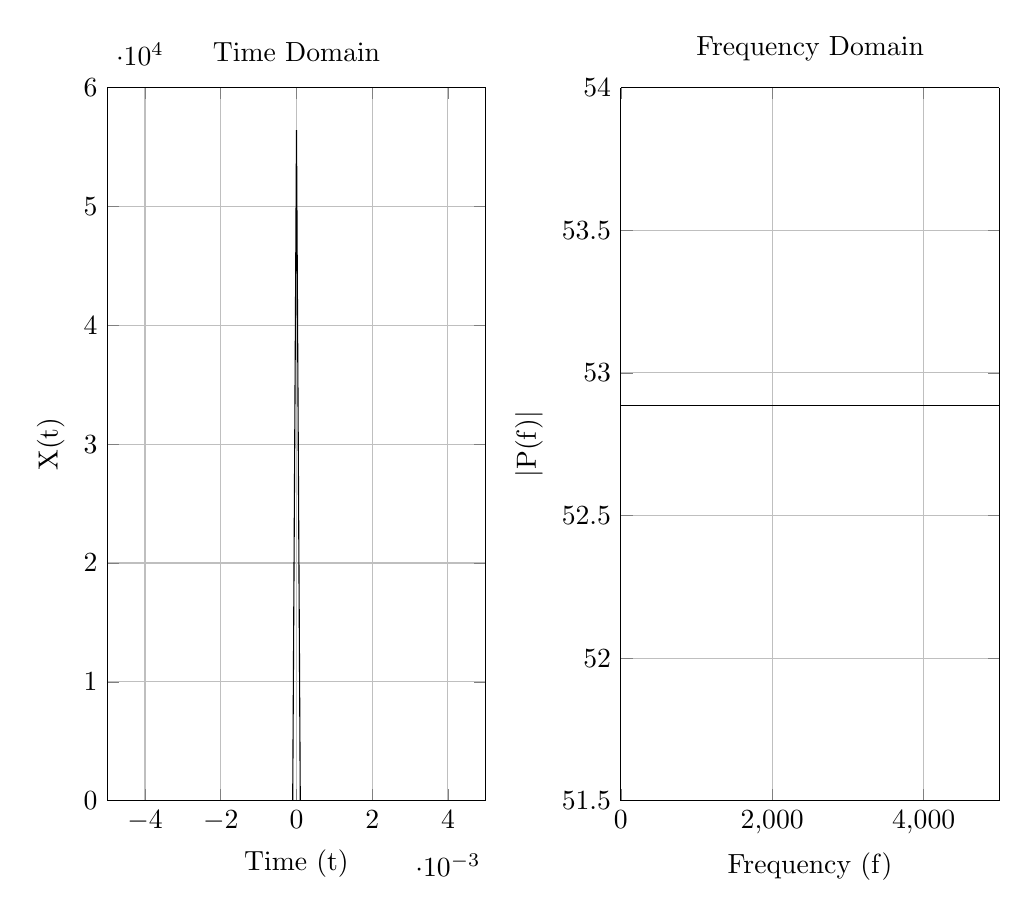
\begin{tikzpicture}

\begin{axis}[%
width=1.893in,
height=3.566in,
at={(0.818in,0.481in)},
scale only axis,
separate axis lines,
every outer x axis line/.append style={black},
every x tick label/.append style={font=\color{black}},
xmin=-0.005,
xmax=0.005,
xlabel={Time (t)},
xmajorgrids,
every outer y axis line/.append style={black},
every y tick label/.append style={font=\color{black}},
ymin=0,
ymax=60000,
ylabel={X(t)},
ymajorgrids,
axis background/.style={fill=white},
title={Time Domain}
]
\addplot [color=black,solid,forget plot]
  table[row sep=crcr]{%
-0.005	0\\
-0.0049	0\\
-0.0048	0\\
-0.0047	0\\
-0.0046	0\\
-0.0045	0\\
-0.0044	0\\
-0.0043	0\\
-0.0042	0\\
-0.0041	0\\
-0.004	0\\
-0.0039	0\\
-0.0038	0\\
-0.0037	0\\
-0.0036	0\\
-0.0035	0\\
-0.0034	0\\
-0.0033	0\\
-0.0032	0\\
-0.0031	0\\
-0.003	0\\
-0.0029	0\\
-0.0028	0\\
-0.0027	0\\
-0.0026	0\\
-0.0025	0\\
-0.0024	0\\
-0.0023	0\\
-0.0022	0\\
-0.0021	0\\
-0.002	0\\
-0.0019	0\\
-0.0018	0\\
-0.0017	0\\
-0.0016	0\\
-0.0015	0\\
-0.0014	0\\
-0.0013	0\\
-0.0012	0\\
-0.0011	0\\
-0.001	0\\
-0.0009	0\\
-0.0008	0\\
-0.0007	0\\
-0.0006	0\\
-0.0005	0\\
-0.0004	0\\
-0.0003	0\\
-0.0002	1.08051873719493e-169\\
-0.0001	2.09882811567613e-39\\
0	56418.9583547756\\
0.0001	2.09882811567613e-39\\
0.0002	1.08051873719493e-169\\
0.0003	0\\
0.0004	0\\
0.0005	0\\
0.0006	0\\
0.0007	0\\
0.0008	0\\
0.0009	0\\
0.001	0\\
0.0011	0\\
0.0012	0\\
0.0013	0\\
0.0014	0\\
0.0015	0\\
0.0016	0\\
0.0017	0\\
0.0018	0\\
0.0019	0\\
0.002	0\\
0.0021	0\\
0.0022	0\\
0.0023	0\\
0.0024	0\\
0.0025	0\\
0.0026	0\\
0.0027	0\\
0.0028	0\\
0.0029	0\\
0.003	0\\
0.0031	0\\
0.0032	0\\
0.0033	0\\
0.0034	0\\
0.0035	0\\
0.0036	0\\
0.0037	0\\
0.0038	0\\
0.0039	0\\
0.004	0\\
0.0041	0\\
0.0042	0\\
0.0043	0\\
0.0044	0\\
0.0045	0\\
0.0046	0\\
0.0047	0\\
0.0048	0\\
0.0049	0\\
0.005	0\\
};
\end{axis}

\begin{axis}[%
width=1.893in,
height=3.566in,
at={(3.386in,0.481in)},
scale only axis,
separate axis lines,
every outer x axis line/.append style={black},
every x tick label/.append style={font=\color{black}},
xmin=0,
xmax=5000,
xlabel={Frequency (f)},
xmajorgrids,
every outer y axis line/.append style={black},
every y tick label/.append style={font=\color{black}},
ymin=51.5,
ymax=54,
ylabel={$|$P(f)$|$},
ymajorgrids,
axis background/.style={fill=white},
title={Frequency Domain}
]
\addplot [color=black,solid,forget plot]
  table[row sep=crcr]{%
0	52.8843018801013\\
78.125	52.8843018801013\\
156.25	52.8843018801013\\
234.375	52.8843018801013\\
312.5	52.8843018801013\\
390.625	52.8843018801013\\
468.75	52.8843018801013\\
546.875	52.8843018801013\\
625	52.8843018801013\\
703.125	52.8843018801013\\
781.25	52.8843018801013\\
859.375	52.8843018801013\\
937.5	52.8843018801013\\
1015.625	52.8843018801013\\
1093.75	52.8843018801013\\
1171.875	52.8843018801013\\
1250	52.8843018801013\\
1328.125	52.8843018801013\\
1406.25	52.8843018801013\\
1484.375	52.8843018801013\\
1562.5	52.8843018801013\\
1640.625	52.8843018801013\\
1718.75	52.8843018801013\\
1796.875	52.8843018801013\\
1875	52.8843018801013\\
1953.125	52.8843018801013\\
2031.25	52.8843018801013\\
2109.375	52.8843018801013\\
2187.5	52.8843018801013\\
2265.625	52.8843018801013\\
2343.75	52.8843018801013\\
2421.875	52.8843018801013\\
2500	52.8843018801013\\
2578.125	52.8843018801013\\
2656.25	52.8843018801013\\
2734.375	52.8843018801013\\
2812.5	52.8843018801013\\
2890.625	52.8843018801013\\
2968.75	52.8843018801013\\
3046.875	52.8843018801013\\
3125	52.8843018801013\\
3203.125	52.8843018801013\\
3281.25	52.8843018801013\\
3359.375	52.8843018801013\\
3437.5	52.8843018801013\\
3515.625	52.8843018801013\\
3593.75	52.8843018801013\\
3671.875	52.8843018801013\\
3750	52.8843018801013\\
3828.125	52.8843018801013\\
3906.25	52.8843018801013\\
3984.375	52.8843018801013\\
4062.5	52.8843018801013\\
4140.625	52.8843018801013\\
4218.75	52.8843018801013\\
4296.875	52.8843018801013\\
4375	52.8843018801013\\
4453.125	52.8843018801013\\
4531.25	52.8843018801013\\
4609.375	52.8843018801013\\
4687.5	52.8843018801013\\
4765.625	52.8843018801013\\
4843.75	52.8843018801013\\
4921.875	52.8843018801013\\
5000	52.8843018801013\\
};
\end{axis}
\end{tikzpicture}%}
\caption{Impulse 1}
\label{fig:impulse1}
\end{subfigure}
\hspace{6mm} 
\begin{subfigure}[t]{0.47\textwidth}
\centering
\tikzsetnextfilename{Impulse2}
\scalebox{0.6}{
% This file was created by matlab2tikz.
%
%The latest updates can be retrieved from
%  http://www.mathworks.com/matlabcentral/fileexchange/22022-matlab2tikz-matlab2tikz
%where you can also make suggestions and rate matlab2tikz.
%
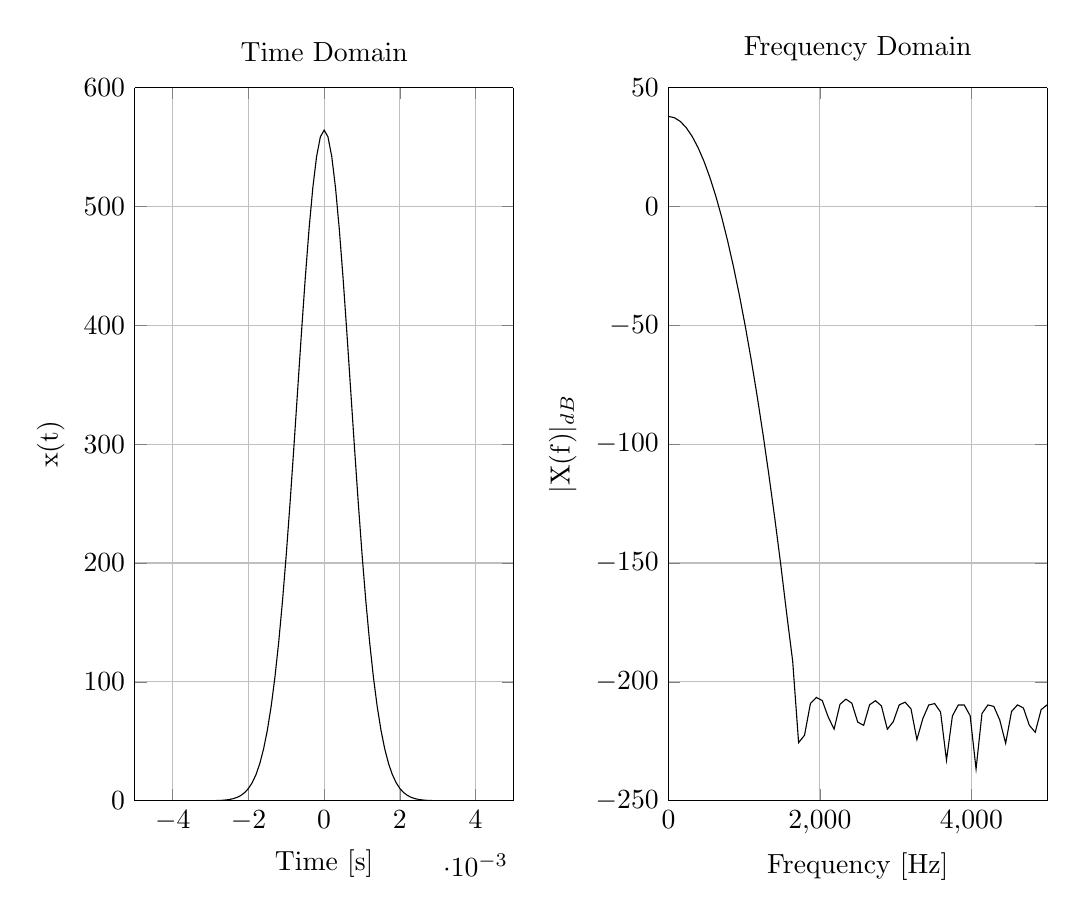
\begin{tikzpicture}

\begin{axis}[%
width=1.893in,
height=3.566in,
at={(0.818in,0.481in)},
scale only axis,
separate axis lines,
every outer x axis line/.append style={black},
every x tick label/.append style={font=\color{black}},
xmin=-0.005,
xmax=0.005,
xlabel={Time [s]},
xmajorgrids,
every outer y axis line/.append style={black},
every y tick label/.append style={font=\color{black}},
ymin=0,
ymax=600,
ylabel={x(t)},
ymajorgrids,
axis background/.style={fill=white},
title={Time Domain}
]
\addplot [color=black,solid,forget plot]
  table[row sep=crcr]{%
-0.005	7.83543326550864e-09\\
-0.0049	2.1086988109929e-08\\
-0.0048	5.56263034490542e-08\\
-0.0047	1.43833470140254e-07\\
-0.0046	3.64547250119098e-07\\
-0.0045	9.05652947954342e-07\\
-0.0044	2.2053823473417e-06\\
-0.0043	5.26405106104077e-06\\
-0.0042	1.23160204933418e-05\\
-0.0041	2.82445606028581e-05\\
-0.004	6.34911733593328e-05\\
-0.0039	0.00013989622447875\\
-0.0038	0.000302143144661123\\
-0.0037	0.000639637042267003\\
-0.0036	0.00132729842235829\\
-0.0035	0.00269971338869239\\
-0.0034	0.00538246051834033\\
-0.0033	0.0105186052217902\\
-0.0032	0.0201488177666178\\
-0.0031	0.0378316333982708\\
-0.003	0.0696265259733739\\
-0.0029	0.125605446260365\\
-0.0028	0.222103972102833\\
-0.0027	0.384962379927571\\
-0.0026	0.654025024861641\\
-0.0025	1.08914211517635\\
-0.0024	1.77782434043888\\
-0.0023	2.84450862126268\\
-0.0022	4.4610775324581\\
-0.0021	6.85782499990342\\
-0.002	10.333492677046\\
-0.0019	15.2623702177239\\
-0.0018	22.0958616660055\\
-0.0017	31.3555202484342\\
-0.0016	43.6145293169727\\
-0.0015	59.4651446118147\\
-0.0014	79.470853838639\\
-0.0013	104.103993398035\\
-0.0012	133.67217350177\\
-0.0011	168.239798896622\\
-0.001	207.553748710297\\
-0.0009	250.984287120181\\
-0.0008	297.492893128735\\
-0.0007	345.637430205269\\
-0.0006	393.621715857144\\
-0.0005	439.391289467723\\
-0.0004	480.770649419654\\
-0.0003	515.630454809482\\
-0.0002	542.067393552432\\
-0.0001	558.575803394468\\
0	564.189583547756\\
0.0001	558.575803394468\\
0.0002	542.067393552432\\
0.0003	515.630454809482\\
0.0004	480.770649419654\\
0.0005	439.391289467723\\
0.0006	393.621715857144\\
0.0007	345.637430205269\\
0.0008	297.492893128735\\
0.0009	250.984287120181\\
0.001	207.553748710297\\
0.0011	168.239798896622\\
0.0012	133.67217350177\\
0.0013	104.103993398035\\
0.0014	79.470853838639\\
0.0015	59.4651446118147\\
0.0016	43.6145293169727\\
0.0017	31.3555202484342\\
0.0018	22.0958616660055\\
0.0019	15.2623702177239\\
0.002	10.333492677046\\
0.0021	6.85782499990342\\
0.0022	4.4610775324581\\
0.0023	2.84450862126268\\
0.0024	1.77782434043888\\
0.0025	1.08914211517635\\
0.0026	0.654025024861641\\
0.0027	0.384962379927571\\
0.0028	0.222103972102833\\
0.0029	0.125605446260365\\
0.003	0.0696265259733739\\
0.0031	0.0378316333982708\\
0.0032	0.0201488177666178\\
0.0033	0.0105186052217902\\
0.0034	0.00538246051834033\\
0.0035	0.00269971338869239\\
0.0036	0.00132729842235829\\
0.0037	0.000639637042267003\\
0.0038	0.000302143144661123\\
0.0039	0.00013989622447875\\
0.004	6.34911733593328e-05\\
0.0041	2.82445606028581e-05\\
0.0042	1.23160204933418e-05\\
0.0043	5.26405106104077e-06\\
0.0044	2.2053823473417e-06\\
0.0045	9.05652947954342e-07\\
0.0046	3.64547250119098e-07\\
0.0047	1.43833470140254e-07\\
0.0048	5.56263034490542e-08\\
0.0049	2.1086988109929e-08\\
0.005	7.83543326550864e-09\\
};
\end{axis}

\begin{axis}[%
width=1.893in,
height=3.566in,
at={(3.486in,0.481in)},
scale only axis,
separate axis lines,
every outer x axis line/.append style={black},
every x tick label/.append style={font=\color{black}},
xmin=0,
xmax=5000,
xlabel={Frequency [Hz]},
xmajorgrids,
every outer y axis line/.append style={black},
every y tick label/.append style={font=\color{black}},
ymin=-250,
ymax=50,
ylabel={$|$X(f)$|_{dB}$},
ymajorgrids,
axis background/.style={fill=white},
title={Frequency Domain}
]
\addplot [color=black,solid,forget plot]
  table[row sep=crcr]{%
0	37.855800607035\\
78.125	37.3325688284896\\
156.25	35.7628734928005\\
234.375	33.1467146000018\\
312.5	29.4840921501025\\
390.625	24.7750061430162\\
468.75	19.0194565789488\\
546.875	12.2174434575596\\
625	4.36896677915439\\
703.125	-4.52597345561197\\
781.25	-14.4673772518028\\
859.375	-25.4552445897236\\
937.5	-37.4895755234318\\
1015.625	-50.5703699969464\\
1093.75	-64.6976273724835\\
1171.875	-79.8713544451494\\
1250	-96.0915066331747\\
1328.125	-113.358286926916\\
1406.25	-131.671567607568\\
1484.375	-151.019248978027\\
1562.5	-171.606034051156\\
1640.625	-191.298724926027\\
1718.75	-225.533783109023\\
1796.875	-222.456448217508\\
1875	-209.062180332166\\
1953.125	-206.532411589981\\
2031.25	-207.856157758439\\
2109.375	-214.736384202754\\
2187.5	-219.848325923748\\
2265.625	-209.428742938503\\
2343.75	-207.254882215146\\
2421.875	-208.951932664328\\
2500	-216.95411287222\\
2578.125	-218.25310330109\\
2656.25	-209.617667296797\\
2734.375	-207.91133374244\\
2812.5	-210.107422986409\\
2890.625	-219.905291162533\\
2968.75	-216.759195752299\\
3046.875	-209.700318071509\\
3125	-208.524028611558\\
3203.125	-211.338813793137\\
3281.25	-224.263264601684\\
3359.375	-215.446664808203\\
3437.5	-209.718709732226\\
3515.625	-209.118734186728\\
3593.75	-212.682258138089\\
3671.875	-232.924718510278\\
3750	-214.310438871519\\
3828.125	-209.709871268567\\
3906.25	-209.709910487451\\
3984.375	-214.208027867961\\
4062.5	-236.634945273642\\
4140.625	-213.312537485231\\
4218.75	-209.697651144571\\
4296.875	-210.317761964784\\
4375	-215.999627109929\\
4453.125	-225.809711386653\\
4531.25	-212.440350012178\\
4609.375	-209.684317861375\\
4687.5	-210.964704832857\\
4765.625	-218.217317888788\\
4843.75	-221.201021704194\\
4921.875	-211.664214485549\\
5000	-209.679117352519\\
};
\end{axis}
\end{tikzpicture}%}
\caption{Impulse 2}
\label{fig:impulse2}
\end{subfigure}
\caption{Two different impulses and there frequency response.}
\label{fig:impulse}
\end{figure}
Besides the characteristics of the impulse the speaker will act as a low pass filter so the frequency response of an impulse will always resemble the frequency response of \autoref{fig:impulse2} of some sort. However when playing music these impulses will be difficult to estimate through an spectrum analysis, because music in itself can consist of impulses.     


%that occurs at playback. The vibrations occurs because the  If the vibration. the sound radiated from the loudspeaker enclosure